\documentclass{standalone}
\usepackage{tikz-network}

\begin{document}
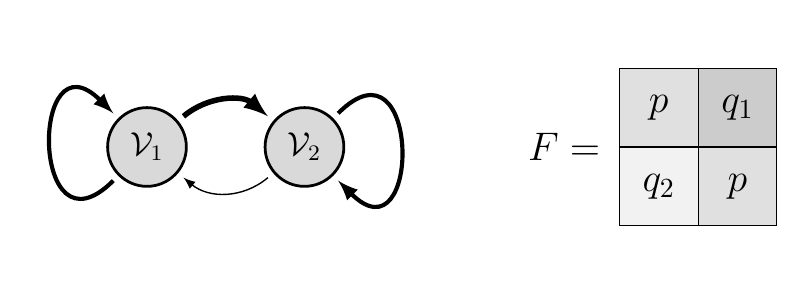
\begin{tikzpicture}

\SetVertexStyle[LineWidth=1, FillColor=black!15!white, LineColor=black, OuterSep=3, TextFont=\large]
\SetEdgeStyle[Color=black]
\SetTextStyle[TextFont=\Large]

\Vertex[label=$\mathcal{V}_1$,size=1]{1}
\Vertex[x=2,size=1,label=$\mathcal{V}_2$]{2}

\Edge[Direct,bend=40,lw=2,position={above=0.1},fontscale=2](1)(2)
\Edge[Direct,bend=40,lw=0.5,position={below=0.1},fontscale=2](2)(1)
\Edge[Direct,loopposition=180,loopsize=1.5cm,position={left=0.1},fontscale=2](1)(1)
\Edge[Direct,loopposition=0,loopsize=1.5cm,position={right=0.1},fontscale=2](2)(2)

\Text[x=5.3,y=0]{$F = $}

\draw[fill=black!12!white] (6,0) rectangle ++(1,1);
\draw[fill=black!20!white] (7,0) rectangle ++(1,1);
\draw[fill=black!5!white] (6,-1) rectangle ++(1,1);
\draw[fill=black!12!white] (7,-1) rectangle ++(1,1);


\Text[x=6.5,y=0.5]{$p$}
\Text[x=7.5,y=0.5]{$q_1$}
\Text[x=6.5,y=-0.5]{$q_2$}
\Text[x=7.5,y=-0.5]{$p$}


\end{tikzpicture}
\end{document}